Sei $ABC$ ein Dreieck und seien $D$, $E$ und $F$ die Höhenfusspunkte der Höhen von $A$, $B$ respektive $C$. Sei $H$ der Höhenschnittpunkt von Dreieck $ABC$. Die Strecken $EF$ und $AD$ schneiden sich in $G$. Sei $K$ der Punkt auf dem Umkreis von Dreieck $ABC$, der diametral gegenüber von $A$ liegt. Die Gerade $AK$ schneide $BC$ in $M$. Zeige, dass die Geraden $GM$ und $HK$ parallel sind.

\begin{center}
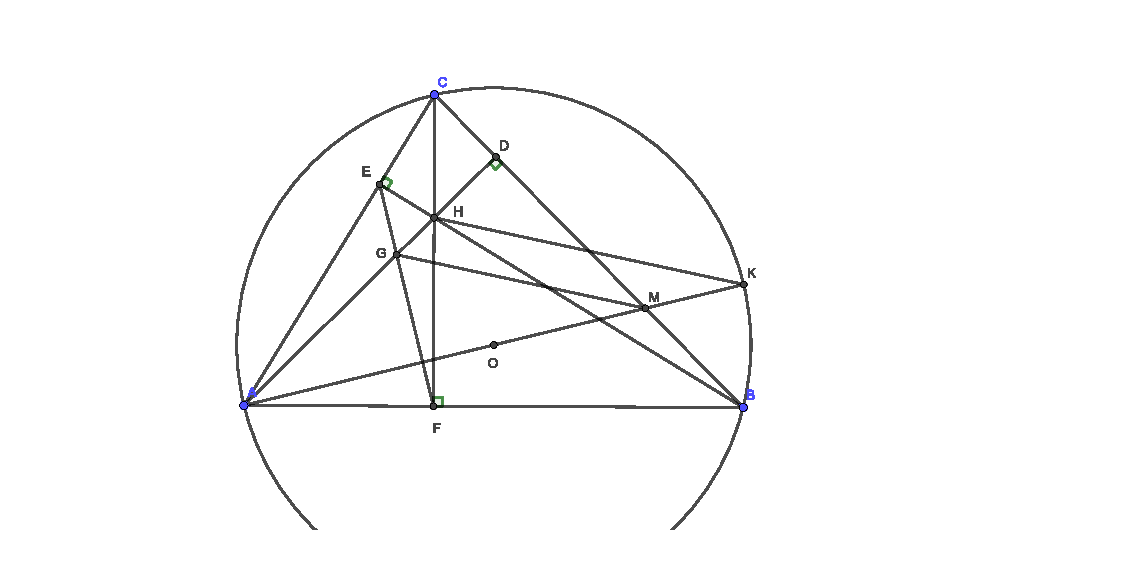
\includegraphics[width=0.85\textwidth,trim=80 60 120 30,  clip]{solutions/s1_picture1.pdf}
\end{center}

\textbf{1. Lösung:} (Cyril)
Wir wollen $GM || HK$ zeigen. Wenn wir annehmen, dass das stimmt und das Ganze von $A$ aus betrachten, können wir das Dreieck $AMG$ zentrisch Strecken, sodass es auf $AKH$ landet. Dies bedeutet, dass wir $\frac{AG}{AH} = \frac{AM}{AK}$ hätten. Die Umkehrung stimmt nun aber auch: Wenn $\frac{AG}{AH} = \frac{AM}{AK}$ gilt, dann sind $GM$ und $HK$ parallel.

Wir wollen also zeigen, dass $\frac{AG}{AH} = \frac{AM}{AK}$ gilt. Dies ist ein Aussage über Verhältnisse, was uns nahelegen kann, dass wir ähnliche Dreiecke suchen sollten. Wenn wir in der Umgebung von $A,G,H$ und $A,M,K$ suchen, dann fällt uns vielleicht der Punkt $E$ und $B$ auf, der in einer sehr "ähnlichen" Lage ist. (wir könnten auch $F$ und $C$ nehmen)

Wir können nun folgende ähnliche Dreieck beweisen: $\triangle AEH \sim \triangle ABK$ und $\triangle EGH = \triangle BMK$. Dafür brauchen wir (i) $\angle AKB = \angle EHA$ und (ii) $\angle ABM = \angle GEA$ und (iii) $\angle KBA = \angle AEH$. (Überprüfe: wenn diese Winkel vorgegeben sind, gibt es nur eine Art, wie wir die Punkte konstruieren können)

\begin{center}
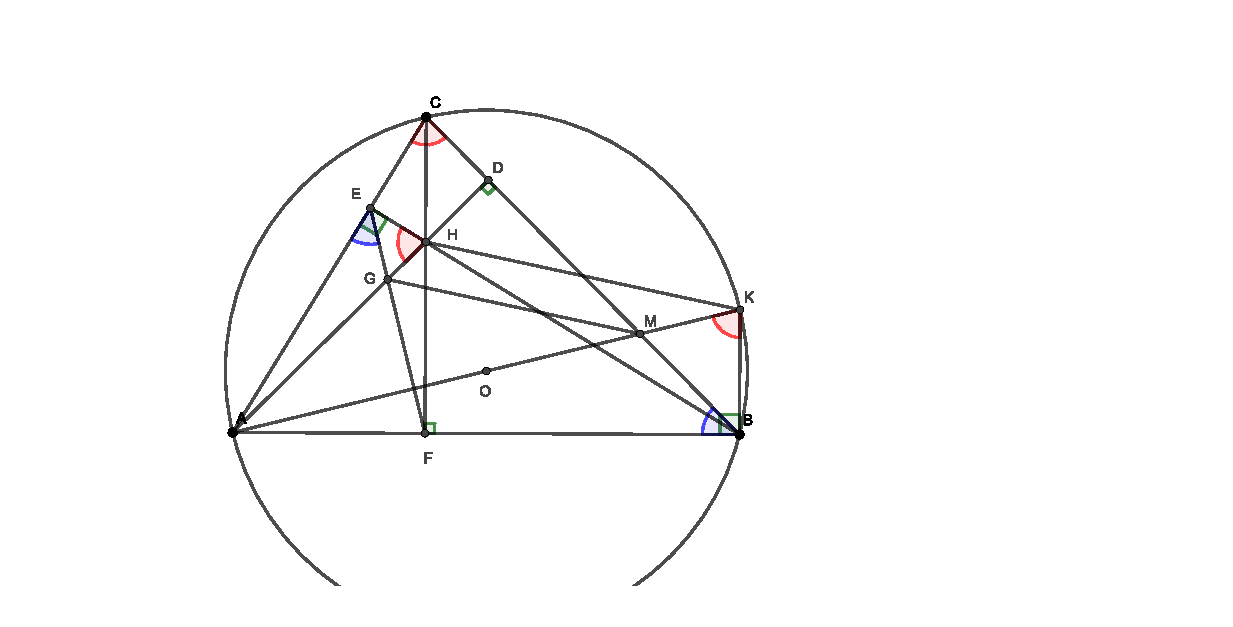
\includegraphics[width=0.85\textwidth,trim=80 60 200 30, clip]{solutions/s1_picture2.pdf}
\end{center}

\begin{enumerate}[(i)]
    \item Wir haben $\angle AKB = \angle BCA$ durch das Sehnenviereck $ABKC$ und $\angle BCA = \angle EHA$ durch das Sehnenviereck $DCEH$
    \item Wir bekommen $\angle ABM = \angle GEA$ direkt wenn wir das Sehnenviereck $BCEF$ betrachten
    \item $\angle KBA = 90^\circ = \angle AEH$ erhalten wir durch Definition des Höhenfusspunktes und $AK$ ein Durchmesser ist
\end{enumerate}
Wir erhalten also $\triangle AEH \sim \triangle ABK$ und damit $\frac{AH}{AK} = \frac{EH}{BK}$. Weiter $\triangle EGH \sim \triangle BMK$ und somit $\frac{EH}{BK} = \frac{GH}{MK}$. Einer der Strahlensätze sagt uns daher, dass $GM || HK$.

\bigskip\bigskip

\textbf{Marking scheme:}
\begin{itemize}
\item 1P: $GM || HK \iff \frac{AG}{AH} = \frac{AM}{AK}$
\item 2P: Ähnliche Dreiecke finden (ohne Beweis)
\item 1P: zwei Winkel in den ähnlichen Dreieck beweisen
\item 1P: dritter Winkel beweisen
\item 1P: Ähnliche Dreiecke $\Rightarrow \frac{AG}{AH} = \frac{AM}{AK}$
\item 1P: fertig
\end{itemize}